\documentclass[aspectratio=169]{beamer}

\usetheme{Madrid}
\usecolortheme{seahorse}

\usepackage[T1]{fontenc}
\usepackage[utf8]{inputenc}
\usepackage[english]{babel}
\usepackage{graphicx}
\usepackage{tikz}
\usetikzlibrary{arrows.meta, positioning, shapes.geometric}

\definecolor{magnusBlue}{HTML}{173F5F}
\definecolor{magnusTeal}{HTML}{206A5D}
\definecolor{magnusGold}{HTML}{F6AE2D}
\definecolor{magnusGray}{HTML}{F3F5F7}

\setbeamercolor{palette primary}{bg=magnusBlue, fg=white}
\setbeamercolor{palette secondary}{bg=magnusTeal, fg=white}
\setbeamercolor{palette tertiary}{bg=magnusGold, fg=black}
\setbeamercolor{frametitle}{bg=magnusBlue, fg=white}
\setbeamercolor{title}{fg=magnusBlue}
\setbeamercolor{block title}{bg=magnusBlue, fg=white}
\setbeamercolor{block body}{bg=magnusGray, fg=black}
\setbeamertemplate{navigation symbols}{}
\setbeamertemplate{footline}{}

\title{Berlin GeoAI Hackathon}
\subtitle{Team Magnus}
\date{10 April - 11 April}

\begin{document}

\begin{frame}[plain,shrink=6]
\vspace{0.08cm}
\noindent
\begin{minipage}[t]{0.10\textwidth}
\vspace{0.02cm}

\includegraphics[width=0.65cm]{HERE_logo.svg.png}
\end{minipage}
\begin{minipage}[t]{0.88\textwidth}
\vspace{0cm}
	{\large \textbf{Berlin GeoAI Hackathon}}\\[-0.02cm]
	{\small Team Magnus \hfill 09 April - 10 April}
\end{minipage}

\vspace{0.02cm}
\begin{center}
	{\large \textbf{Day 1 Summary}}
\end{center}

\vspace{0.01cm}
\setlength{\columnsep}{5mm}
\begin{columns}[T,onlytextwidth,totalwidth=\textwidth]
	\column{0.29\textwidth}
	\begin{block}{Data explored}
	\footnotesize
	\begin{itemize}
		\item Mapped the available Potsdam-Berlin datasets.
		\item Checked school signs, road geometry, and schools.
		\item Linked the 1,850 Mapillary images to the sign workflow.
	\end{itemize}
	\end{block}

	\column{0.36\textwidth}
	\begin{center}
	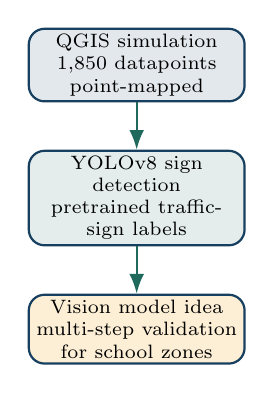
\begin{tikzpicture}[
		node distance=6mm,
		every node/.style={font=\scriptsize},
		box/.style={rounded corners=2mm, draw=magnusBlue, thick, fill=magnusGray, minimum width=2.7cm, minimum height=0.75cm, align=center, text width=2.6cm, inner sep=2pt},
		arrow/.style={-{Latex[length=2.5mm]}, thick, draw=magnusTeal}
	]
		\node[box, fill=magnusBlue!12] (qgis) {QGIS simulation\\1,850 datapoints point-mapped};
		\node[box, below=of qgis, fill=magnusTeal!12] (yolo) {YOLOv8 sign detection\\pretrained traffic-sign labels};
		\node[box, below=of yolo, fill=magnusGold!20] (vision) {Vision model idea\\multi-step validation for school zones};

		\draw[arrow] (qgis) -- (yolo);
		\draw[arrow] (yolo) -- (vision);
	\end{tikzpicture}
	\end{center}

	\column{0.29\textwidth}
	\begin{block}{Pipeline ideation}
	\footnotesize
	\begin{itemize}
		\item Moving from single sign detection to evidence-based validation.
		\item Estimating where a school zone starts and ends from multiple signals.
		\item Handling conditional restrictions like time-based limits.
	\end{itemize}
	\end{block}
\end{columns}

\vfill
\begin{block}{Day 1 outcome}
We now have a clear direction: combine image-based sign detection with geo-data and a multi-step vision validation flow to decide school-zone range, speed limit, and conditional rules.
\end{block}

\end{frame}

\end{document}
